In this chapter, we present our proposed methodology, including the methods and techniques used to address our research questions. We also cover our data exploration and preprocessing steps, the hyperparameter tuning process, and the automated and human evaluation methods and metrics we have chosen.

\section{Data exploration, preprocessing and augmentation}
\subsection{Exploratory data analysis}
First, an exploratory data analysis (EDA) will be conducted to understand the characteristics of the OpenML dataset descriptions. This analysis will be unstructured, discovering patterns in the data in an exploratory manner, using statistical and visual methods. The goal of the EDA is to gain insights into the dataset descriptions, such as their length, vocabulary, distribution of words, etc. This information will help us understand the nature of the data and identify any preprocessing steps that may be necessary to improve the quality of the descriptions.

\subsection{Data preprocessing}
After the EDA, the dataset descriptions will undergo preprocessing to prepare them for the topic modeling process. This preprocessing may involve steps such as stemming, lemmatization, stop-word removal, and tokenization. These steps are important to ensure that the descriptions are in a suitable format for the topic modeling algorithms.

\subsection{Data augmentation}
In addition to the original dataset descriptions, we will explore the possibility of augmenting the data with additional information. This could include metadata such as dataset name, tags, features (column names), scraping from the original dataset if available, etc. This additional information can provide context and background to the descriptions, which may help improve the quality of the topics extracted by the topic model.

\section{Tag generation}
In this subsection, we introduce our model, which is, in fact, a pipeline comprising multiple submodels and techniques. Steps 1-3 involve data preprocessing to prepare the data for the model. Steps 5-8 are referred to as the \textit{Base BERTopic model}. It includes dimensionality reduction, clustering, bag-of-words and c-TF-IDF. Finally, steps 9 and 10 represent our improvements to the base model, introducing an approach that, to the best of our knowledge, is novel within the literature. Additionally, we provide an explanation of which steps are computationally efficient and which are more expensive.

\begin{figure}[h]
    \centering
    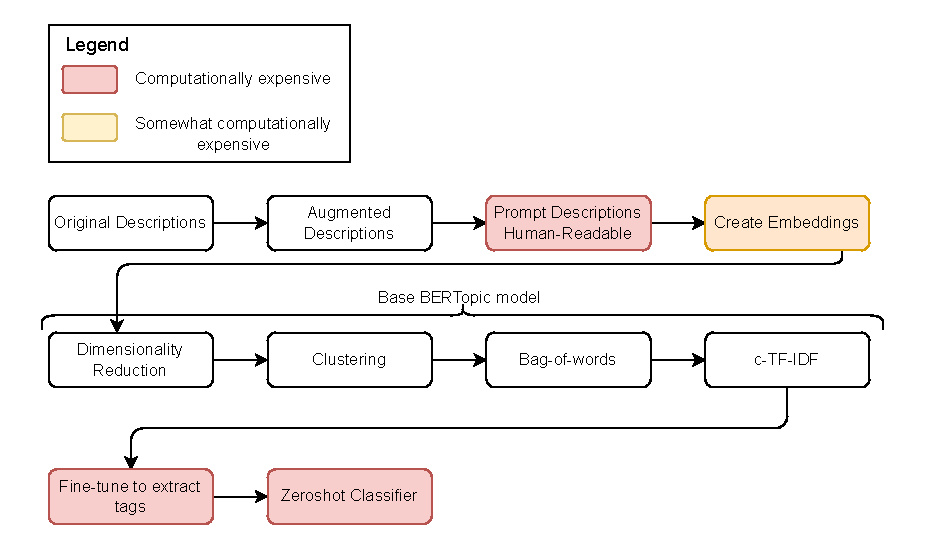
\includegraphics[width=\textwidth]{figures/tag_generation_pipeline.pdf}
    \caption{Tag generation pipeline}
    \label{fig:tag_generation_pipeline}
\end{figure}

To explain the pipeline illustrated in \cref{fig:tag_generation_pipeline} in more detail, we provide a step-by-step description of the process:

\begin{enumerate}
    \item \textbf{Original Descriptions}: The input to the pipeline is a set of original dataset descriptions. These come from the OpenML dataset and are used as the basis for generating tags.
    \item \textbf{Augmented Descriptions}: The OpenML dataset descriptions come with metadata such as dataset name, tags, features (column names) and some of them link to the original dataset, which can be used to scrape (extract) additional information. These are used to augment the dataset descriptions.
    \item \textbf{Prompt Descriptions Human-Readable}: Augmented descriptions are rewritten to be more human-readable via an LLM and prompt engineering. This is because the original descriptions are often in a technical format that is not easily interpretable by humans. Since LLMs are trained on large text corpora, they work best with human-readable (natural language) text.
    
    Additionally, we design the prompt to extract \textit{keyword tags} from each individual description. These tags are directly mentioned within the description and are typically highly specific to it. For instance, if a description includes the terms "US elections," "voting," and "candidates," these would be considered keyword tags.

    \item \textbf{Create Embeddings}: Embeddings for each description are created using a pre-trained embedding model.
    \item \textbf{Dimensionality Reduction}: The dimensionality of the embeddings is reduced to cure the curse of dimensionality.
    \item \textbf{Clustering}: The reduced embeddings are clustered to group similar descriptions together. The output of this step is clusters, which represent our topics. Each cluster contains a set of descriptions (which we now call \textit{representative documents}) that are similar to each other.
    \item \textbf{Bag-of-words}: The descriptions in each cluster are converted to a bag-of-words representation, ignoring common words such as "the", "and", etc.
    \item \textbf{c-TF-IDF}: The bag-of-words representation is used to calculate the c-TF-IDF score for each word in each cluster. This score is used to rank the words in each cluster.
    \item \textbf{Fine-tune to extract tags}: For each topic, we have representative documents (from the clustering step) and representative words (from the c-TF-IDF step). We prompt engineer a question that asks an LLM to generate tags for each cluster. The generated tags are categorized as \textit{regular tags} and \textit{overarching tags}.

    \textit{Regular tags} refer to tags that frequently appear among the representative documents and words. \textit{Overarching tags} capture the broader, more general theme of the cluster. For example, if a cluster pertains to "US elections" and the representative documents contain the word "election" while the representative words include "candidate", a possible regular tag could be "election candidate", whereas the overarching tag might be "politics".

    As context, we feed the LLM with the top \textit{k} representative documents and the top \textit{m} representative words for each topic. This results in tags that are common among the representative documents and representative words, and hence are representative of the topic.
    \item \textbf{Zeroshot Classifier}: Each description can in reality be contained in multiple clusters (topics). In this step, we get the top \textit{n} most likely clusters for each description. Then, for each description, we get the tags for each of the top \textit{n} clusters in a set. We feed this set of tags to a zeroshot text classification model, which returns confidences from 0 to 1 for whether each tag describes the description. This step is crucial for filtering out irrelevant tags for each description. For instance, if a description about diabetes and a description about cancer are both contained in the same topic (which may be, for example, "medical conditions"), we want to ensure that the tags for the cancer description are not assigned to the diabetes description. Furthermore, the description about diabetes may be contained in another topic that cancer is not in, such as "nutrition". In this case, we want to ensure that the tags in "nutrition" are not assigned to the cancer description, but are assigned to the diabetes description.

\end{enumerate}


\section{Automated evaluation metrics, baselines}
In order to evaluate the quality of the extracted topics, we will use a combination of automated evaluation metrics and baselines. These metrics and baselines will help us assess the performance of our model and compare it to existing topic modeling techniques. The following sections provide an overview of the metrics and baselines we will use in our evaluation.

\subsection{Metrics}
\subsubsection{Topic coherence}
As explained in \cref{sec:topic_coherence}, topic coherence is a widely used metric for evaluating the quality of topics generated by topic models. It measures the semantic similarity between words in a topic and is based on the assumption that coherent topics contain words that are related to each other. We will use topic coherence to assess the quality of the topics extracted by our model.

\subsubsection{Topic diversity}
Topic diversity (\cref{sec:topic_diversity}) is another important metric for evaluating topic models. It measures the extent to which topics are distinct from each other and do not overlap in terms of the words they contain. A diverse set of topics ensures that the model captures a wide range of themes and concepts present in the data. We will use topic diversity to evaluate the diversity of topics generated by our model.

\subsubsection{Silhouette score}
The silhouette score (\cref{sec:silhouette_score}) is a metric used to evaluate the quality of clusters in unsupervised learning. It measures how similar an object is to its own cluster (cohesion) compared to other clusters (separation). A high silhouette score indicates that the clusters are well-separated and that the objects within each cluster are similar to each other. We will use the silhouette score to evaluate the quality of the clusters generated by our model.

\subsection{Baselines}
In addition to the proposed topic model, we will compare its performance against several baseline models. These baselines represent established or commonly used topic modeling techniques and will serve as a point of reference for evaluating the proposed model. The baselines we will consider include Latent Dirichlet Allocation (LDA), Non-negative Matrix Factorization (NMF), and Top2Vec (described in \cref{sec:latent_dirichlet_allocation,sec:non-negative_matrix_factorization,sec:top2vec}). These models are widely used in the field of topic modeling and will provide a benchmark for evaluating the performance of our model.

\subsection{Automated evaluation pipeline}

\Cref{fig:data_pipeline} shows a flowchart of the automated evaluation pipeline, which contains the following sequential steps:

\begin{enumerate}

    \item \textbf{Data Fetching}: This is the first stage where dataset descriptions are downloaded from OpenML.

    \item \textbf{Data Preparation}: After fetching the data, the next step involves preparing it. This includes removing noise, correcting errors, augmenting it, and standardizing the format to prepare it for analysis. Data preparation ensures that the input to the topic model is of high quality, which is crucial for the success of the subsequent modeling steps. \\ The next step involves removing inadequate data points, such as excessively short descriptions and duplicates. Stop words are removed for models that require it (e.g., LDA). Additionally, the process includes stemming and lemmatization to normalize words to their base forms.

    \item \textbf{Topic Model}: In this step, the proposed topic model is applied to the prepared data. In this case, it will be BERTopic. We refer to it as the \textit{Base BERTopic model}.

    \item \textbf{Benchmark Models}: Concurrently with the proposed topic model, benchmark models are run. These models represent established or baseline approaches to topic modeling against which the performance of the proposed topic model is compared. This will involve baseline models such as LDA, NMF and Top2Vec.

    \item \textbf{Topic Labels}: The output from both the topic model and the benchmark models are sets of topics, represented by a cluster of words that are characteristic of a particular topic.

    \item \textbf{Evaluation}: Finally, the performances of the proposed topic model and benchmark models are evaluated. This includes comparing the topic coherence, diversity and silhouette score.

\end{enumerate}

\begin{figure}[h]
    \centering
    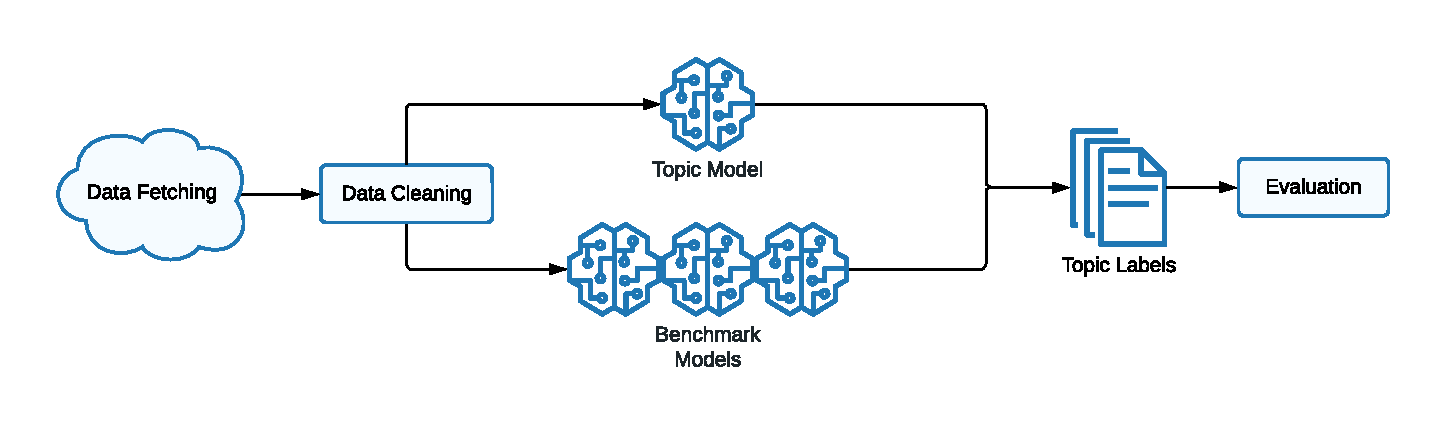
\includegraphics[width=\textwidth]{figures/data_pipeline.pdf}
    \caption{Data pipeline}
    \label{fig:data_pipeline}
\end{figure}

\subsection{Hyperparameter tuning}
As mentioned in \cref{sec:octis}, we will use Bayesian optimization to tune the hyperparameters of our \textit{Base BERTopic model}. This process will involve selecting the most relevant hyperparameters to optimize, defining the search space for each hyperparameter, and running the optimization algorithm to find the best combination of hyperparameters. The goal of hyperparameter tuning is to improve the performance of our model by finding the settings for the hyperparameters which are close to optimal.

As a metric to optimize, we will use the topic coherence score, which is a widely used measure of topic quality in topic modeling. By maximizing the topic coherence score, we aim to find the hyperparameters that produce the most coherent and interpretable topics. The hyperparameters we will tune include the number of topics, the parameters of the dimensionality reduction algorithm, the clustering algorithm, etc.

\section{Human evaluation}
After designing our pipeline, we will perform a human evaluation to assess the quality of the tags produced by our model. As previously discussed, automated evaluation metrics offer only a limited perspective on the quality of the generated tags. Human evaluation is crucial for providing a more comprehensive assessment. To this end, we will carry out a user study in which participants will evaluate the quality of the tags generated by our model.

\subsection{Experimental design}
\subsubsection{Research questions}
Our human evaluation aims to address the following research questions:

\begin{itemize}
\item Q1. Is the model good at generating individual tags relevant to the themes in the documents (\textit{relevance})?
\item Q2. Is the model good at producing a good distribution between specific tags and general tags per document (\textit{generality})?
\item Q3. Is the model good at covering the range of themes in the document (\textit{coverage})?
\item Q4. Is the model good at capturing common tags between documents (\textit{shared coverage})?
\item Q5. Does the model exhibit \textit{robustness} by consistently producing high-quality tags across different documents and domains?
\end{itemize}

Questions Q1-Q4 will be directly addressed through our human evaluation tasks. Q5 is a broader question that our study will provide insights into, although a comprehensive answer to this question may require additional research beyond the scope of this evaluation.

\textit{Robustness} in this context refers to the model's ability to consistently generate relevant, specific, general, and comprehensive tags across a wide range of documents and domains. While our study will provide initial insights into robustness, fully addressing this question would require evaluation across a larger and more diverse set of OpenML datasets.

\subsubsection{Evaluation criteria}
Participants will evaluate tags based on four main criteria, each addressing a specific research question:

\begin{itemize}
\item \textit{Relevance} (Q1): How well each tag represents the main themes of the document, rated on a 1-5 scale:
\begin{itemize}
\item 1 - Not at all
\item 2 - Somewhat well
\item 3 - Moderately well
\item 4 - Very well
\item 5 - Extremely well
\end{itemize}
Example: A document about Covid-19 with tags \textit{Covid-19}, \textit{Virus}, \textit{Car Crash}

\item \textit{Generality} (Q2): How general or specific the tag is to the particular document, rated on a 1-5 scale:
\begin{itemize}
\item 1 - Very specific to this document
\item 2 - Somewhat specific
\item 3 - Balanced
\item 4 - Somewhat general
\item 5 - Very general, could apply to many documents
\end{itemize}
Example: A document about Covid-19 with tags \textit{Covid-19}, \textit{Virus}, \textit{Medicine}, \textit{Science}

\item \textit{Coverage} (Q3): How well the set of tags covers the range of themes within the document, rated on a 1-5 scale. If a participant does not rate this as 5, they will be prompted to suggest additional tags that would improve coverage.
Example: A document about Covid-19 Biotechnology Companies with tags \textit{Covid-19}, \textit{Virus}, \textit{Medicine}, \textit{Science} (but missing \textit{Biotechnology})

\item \textit{Shared Coverage} (Q4): How well the common tags represent shared themes between two documents, rated on a 1-5 scale.
Example: For datasets about Covid-19 Biotechnology Companies and Covid-19 World Vaccination Progress, common tags might include \textit{Covid-19}, \textit{Virus}, \textit{Medicine} (but not \textit{Biotechnology} or \textit{Vaccinations})
\end{itemize}

The goal is to measure relevance and coverage (higher is better), and to assess the distribution of generality (a large standard deviation is desirable, indicating a good mix of specific and general tags). Shared coverage aims to evaluate the model's ability to capture common themes across related documents, which is crucial for dataset discoverability.

\subsubsection{Participants}
We will begin by recruiting participants for the user study. Given that participants will be selected based on accessibility, this will constitute a convenience sample. Colleagues, friends, and acquaintances will be invited to participate. Despite the use of a convenience sample, we will aim to recruit individuals whose backgrounds align with those of OpenML's target users. Specifically, we will seek participants with expertise in data science, computer science, or, at a minimum, individuals with a bachelor's degree and a high proficiency in English.

\subsubsection{Materials}
The study will utilize selected OpenML dataset descriptions as documents. Three separate surveys will be created, each containing the same set of documents but with different sets of tags:

\begin{enumerate}
\item A survey with tags generated by the \textit{proposed model}
\item A survey with tags generated by the \textit{baseline model}
\item A survey with \textit{human-generated tags}
\end{enumerate}

This design allows for a direct comparison of tag quality across different tag generation methods while keeping the document content constant. Data collection will be facilitated through Google Forms, with each survey distributed to a subset of participants. Python will be used for subsequent data analysis.

The use of identical documents across all three surveys ensures that any differences in tag evaluation can be attributed to the tag generation method rather than variations in document content. This approach will provide insights into the relative performance of the proposed model compared to both a baseline model and human-generated tags.

\subsubsection{Variables}
Our experimental design involves several types of variables:

\paragraph{Independent Variables (IVs):}
The primary independent variable in this study is the \textit{Tag Set}. This refers to the different sets of tags provided to participants for rating across the three surveys (proposed model, baseline model, and human-generated tags). We will investigate how these different tag sets impact the dependent variables.

\paragraph{Dependent Variables (DVs):}
The dependent variables are the outcomes we are measuring, specifically the ratings participants provide for the tags. These include:
\begin{itemize}
\item Relevance ratings
\item Generality ratings
\item Coverage ratings
\item Shared coverage ratings
\end{itemize}

\paragraph{Controlled Variables (CVs):}
To ensure the validity of our comparisons, we will control the following variables:
\begin{itemize}
\item \textit{Texts}: The same dataset descriptions will be used across all surveys.
\item \textit{Survey Structure}: The instructions, layout, and format will be consistent across all surveys.
\item \textit{Rating Scale}: The same 1-5 scale will be used for all rating tasks.
\item \textit{Participants}: While not all participants will complete all surveys due to resource constraints, we will ensure that the participant pools for each survey are comparable in terms of expertise and background.
\end{itemize}

By manipulating the independent variable (Tag Set) while controlling for other factors, we aim to isolate the effect of different tag generation methods on the quality of tags as perceived by human evaluators.

\subsubsection{Procedure}
The experiment will be conducted in two stages: \textit{Individual Document Evaluation} and \textit{Document Pair Evaluation}.

In the first stage, participants will perform two tasks:

The \textit{Intruder Detection Task} will present participants with a document and a set of tags, including one intruder tag, which they must identify. \textit{Intruder Detection} is a common task in topic modeling studies, where human evaluators are asked to identify the term that does not belong to the topic \cite{chang_reading_2009, newman_evaluating_2010, musil_exploring_2024, lau_machine_2014, bhatia_automatic_2017, hoyle_is_2021}.
The \textit{Tag Quality Assessment Task}, where participants will rate each tag on its relevance and generality using 1-5 scales, as well as rate the overall coverage of the tag set.
The second stage, \textit{Document Pair Evaluation}, also consists of two tasks:

In the \textit{Common Tags Identification Task}, participants will be presented with two related documents and their respective tag sets, and asked to identify the common tags between the two sets.
This will be followed by the \textit{Common Tags Quality Assessment Task}, where participants will rate the shared coverage of the common tags using a 1-5 scale.
These tasks are designed to address the specific research questions:

\begin{itemize}
\item The \textit{Intruder Detection Task} and \textit{Tag Quality Assessment Task} address Q1 (relevance), Q2 (generality), and Q3 (coverage).
\item The \textit{Common Tags Identification Task} and \textit{Common Tags Quality Assessment Task} address Q4 (shared coverage).
\end{itemize}

Additionally, these tasks will help evaluate:

\begin{itemize}
\item \textit{Robustness}: If the model consistently produces pairs of tag sets for related documents where the intersection is easily identifiable, demonstrating robustness in tag generation across documents.
\end{itemize}

It is important to note that while this human evaluation provides valuable insights, it cannot fully address questions of robustness across all OpenML datasets due to resource constraints. The evaluation of consistent performance across a large number of datasets remains a challenge for future work.

\subsubsection{Data collection}
Data will be collected through Google Forms. Participants will submit their responses for each task, including identified intruder tags, relevance and generality ratings for individual tags, coverage ratings for tag sets, identified common tags between document pairs, and shared coverage ratings for common tags.

\subsubsection{Analysis plan}
The analysis will encompass a range of statistical techniques to evaluate the performance of the proposed model. We will calculate true positive and false positive rates for intruder detection, and compute average relevance, generality, and coverage scores. The distribution of these scores will be analyzed to understand the spread and variability of the ratings.

Correlation analysis will be performed to explore relationships between relevance, generality, and coverage. We will also compare scores between regular tags, overarching tags, and keyword tags to identify any significant differences.

For the common tag identification task, we will calculate true positive, true negative, false positive, and false negative rates. Inter-rater reliability analysis will be conducted to assess the consistency of ratings across participants. Hypothesis testing will be employed to compare group means, medians or variances, and effect sizes will be calculated to quantify the magnitude of any differences found.

\subsubsection{Ethical considerations}
All participants will be provided with clear information about the study's purpose and procedures, and their informed consent will be obtained before participation. Data privacy will be ensured by anonymizing and securely storing participant responses. Participants will be informed of their right to withdraw from the study at any time without penalty.

The study poses minimal risk to participants as it involves only text evaluation tasks. If applicable, participants will be fairly compensated for their time and effort, ensuring that the study adheres to ethical standards of research conduct.

\subsubsection{Limitations}
Several limitations of this study should be acknowledged. The use of a convenience sample may limit the generalizability of the results. The evaluation of tags involves subjective judgments, which may introduce some variability in the results. The study focuses on a specific set of documents and may not cover all possible domains or types of datasets.

Resource constraints may limit the number of participants and documents evaluated. Additionally, the study provides a snapshot of tag quality but does not assess the long-term usefulness of the tags in real-world scenarios. These limitations should be considered when interpreting the results and drawing conclusions from the study.

Furthermore, while the study aims to provide insights into the model's robustness, the limited scope of the evaluation means that we cannot fully assess the model's performance across all OpenML datasets. This remains an area for potential future research.

\subsubsection{Hypotheses}
We propose the following hypotheses for this study:

The \textit{proposed model} will generate tags with higher relevance scores compared to the baseline model. We expect to see a more balanced distribution of general and specific tags from the proposed model compared to the baseline model. The coverage scores for the proposed model's tag sets are hypothesized to be significantly higher than those of the baseline model.

Furthermore, we anticipate that the shared coverage scores for the proposed model's common tags will be significantly higher than those of the baseline model. We hypothesize a positive correlation between tag relevance and coverage scores. Finally, we expect some inter-rater reliability for tag evaluations, indicating somewhat consistent judgments across participants.

These hypotheses will guide our analysis and help us evaluate the effectiveness of the proposed model in generating high-quality, relevant, and comprehensive tags for dataset descriptions.

\subsection{Large-scale Automated Evaluation}

To complement our human evaluation and to assess the model's performance across a larger number of OpenML datasets, we propose using a large language model (LLM) as a proxy for human evaluators. This approach is inspired by recent literature demonstrating the effectiveness of LLMs in simulating human judgments for certain tasks \cite{musil_exploring_2024}.

We will use GPT-4-mini to evaluate all available OpenML dataset descriptions, both with tags generated from the baseline model and tags generated by the proposed model. This automated evaluation will consist of two main tasks.

\subsubsection{Automated Intruder Detection}
For each OpenML dataset description, we will present the LLM with the description and a set of tags, including one intruder tag. The LLM will be tasked with identifying the intruder tag.

\subsubsection{Automated Tag Quality Assessment}
For each dataset, we will prompt the LLM to rate the relevance, generality, and coverage of the tags using the same 1-5 scale as in the human evaluation.

\subsubsection{Rationale}
This large-scale automated evaluation will allow us to assess the model's performance across a much larger and more diverse set of datasets, providing insights into the model's robustness and consistency. Additionally, it will enable us to generate a large amount of evaluation data quickly and cost-effectively.

However, it's important to note the limitations of this approach. LLMs, while sophisticated, are not perfect proxies for human judgment. The automated evaluation will not include the document pair tasks from the human evaluation, as the number of possible combinations of document pairs is prohibitively large ($O(n^2)$ for $n$ documents), limiting our ability to assess shared coverage across datasets. Moreover, the results may be influenced by biases inherent in the LLM's training data.

The results from this automated evaluation will be analyzed in conjunction with the human evaluation results to provide a more comprehensive assessment of our model's performance. This dual approach of human and automated evaluation will offer a multifaceted understanding of our model's capabilities and limitations in generating high-quality tags for OpenML dataset descriptions.

\section{Chapter summary}
This chapter addresses several of our research questions. \hyperref[rq1]{\textbf{RQ1}} is partially answered through our proposed data exploration, preprocessing and augmentation steps, which will help us understand the characteristics of OpenML dataset descriptions and their potential impact on model performance.

\hyperref[rq2]{\textbf{RQ2}} is addressed by our novel tag generation pipeline, which builds upon the BERTopic model and incorporates additional steps for fine-tuning and tag filtering.

\hyperref[rq3]{\textbf{RQ3}} and \hyperref[rq4]{\textbf{RQ4}} are tackled through our evaluation strategy, which includes both automated metrics and a detailed human evaluation plan. We have outlined specific metrics and procedures for assessing the quality and usefulness of the generated tags.

Additionally, we have proposed a large-scale automated evaluation using a language model as a proxy for human judgment, which further contributes to addressing \hyperref[rq3]{\textbf{RQ3}} and \hyperref[rq4]{\textbf{RQ4}}.